
\chapter[Numerical Methods for the System of Equations
  of...]{Numerical Methods for the System of Equations of 
  Hydrodynamics - Lagrangian Coordinates}\label{chap9} 

\section{Introduction}\label{chap9:sec9.1}

We\pageoriginale now study the approximation of the system of
equations of hydrodynamics in the slab-symmetric, 1-dimensional case,
in the Lagrangian framework. We will esentially use the leap-frog
scheme in discretizing these equations. We will also discuss the
question of boundary conditions  and the pseudo-viscosity term and
present a heuristic discussion of stability criteria. 

With $\mu = 0$ and $g= 0$, the equations fo hydrodynamics assume the form 
\begin{equation*}
\frac{D\rho}{Dt} + \rho \frac{\partial u}{\partial x} = 0\tag{9.1}\label{eq9.1}
\end{equation*}
or, equivalently,
\begin{gather*}
\frac{D }{D t} (\rho J) = 0 \tag*{$(9.1')$}\label{eq9.1'}\\
\frac{D u}{D t} + \frac{1}{\rho} \frac{\partial p}{\partial x} = 0, \text{ and } \tag{9.2}\label{eq9.2}\\
\frac{D \epsilon}{D t } + p \frac{D}{D t} \left(\frac{1}{\rho}\right) -
\frac{1}{\rho}  \frac{1}{\rho} \frac{\partial}{\partial x} \left(k
\frac{\partial T}{\partial x}\right) = 0 \tag{9.3}\label{eq9.3}  
\end{gather*}
(Note: We recall our comments on the Lagrangian form of the equation made in section \ref{chap1:sec1.5}. To be strictly Lagrangian in formulation, $x$ must be expressed in terms of $a$).

\section{Leap-Frog scheme for the isentropic case}\label{chap9:sec9.2}

We assume for the time being that $k=0$ and also that (\ref{eq9.3}) can be integrated to get $p$ in terms of $\rho$, i.e. $p = p (\rho)$. (Example: The isentropic case of a perfect gas gives $p=c \rho^\gamma$) Then we are left with (\ref{eq9.1}) and (\ref{eq9.2}) to discretize.

Recalling\pageoriginale our definition of $m$
(Cf. Sec. \ref{chap2:sec2.3}) one can take as space variable either
$a$ or $m$. In using the leap-frog scheme one notes an essential
property of this scheme: when dealing with a hyperbolic system such as
(\ref{eq9.1}) and (\ref{eq9.2}) one need not compute all the unknowns
at all the nodes  of the mesh. One case compute certain unknowns on
some of the nodes and the others at the remaining nodes. Thus here one
computes $\rho$ and $p$ at the nodes $\left(i+\frac{1}{2}, n\right)$ and the
velocity $u$ at the nodes $(i, n+\frac{1}{2})$. 

We approximate the equation defining $u$ as $\dfrac{dx}{dt}$ by.
\begin{equation*}
x^{n+1}_i = x^n_i + u^{n+\frac{1}{2}}_i \Delta t \tag{9.4}\label{eq9.4}
\end{equation*}
where $x^\circ_i$, is the same as the $a_i$ chosen at the horizontal axis. (Note that (\ref{eq9.4}) merely gives discretization of the relation between the Eulerian and Lagrangian coordinates). Then the equation (\ref{eq9.1'}) says that the mass contained between $x^{n+1}_{i+1}$ and $x^{n+1}_i$ is independent of time, i.e. $n$. Hence we can write 
\begin{equation*}
\rho^{n+1}_{i+\frac{1}{2}} (x^{n+1}_{i+1} - x^{n+1}_i) = \text{ Const. } = \Delta m_{i+\frac{1}{2}} = \rho^n_{i+\frac{1}{2}} (x^n_{i+1} - x^n_i)\tag{9.5}\label{eq9.5}
\end{equation*}
as a discretization of (\ref{eq9.1'}) assuming $\rho$ constant in this interval.

Actually (\ref{eq9.4}) and (\ref{eq9.5}) which are the discretizations of (\ref{eq9.1'}) imply the following which can be thought as a discretization of (\ref{eq9.1})
\begin{equation*}
\frac{\rho^{n+1}_{i+\frac{1}{2}} - \rho^n_{i+\frac{1}{2}}}{\Delta t} + \frac{1}{2}
 (\rho^{n+1}_{i+\frac{1}{2}} + \rho^n_{i+\frac{1}{2}})  \frac{(u^{n+\frac{1}{2}}_{i+1} - u^{n+\frac{1}{2}}_i)}{(\frac{1}{2} (x^{n+1}_{i+1} + x^n_{i+1}) -\frac{1}{2} (x^{n+1}_i + x^n_i))} =0.\tag{9.6}\label{eq9.6}
\end{equation*}

If we define 
\begin{equation*}
\Delta m_i = \frac{1}{2} (\Delta m_{i+\frac{1}{2}} + \Delta m_{i-\frac{1}{2}})\tag{9.7}\label{eq9.7}
\end{equation*}
one can discretize (\ref{eq9.2}) by
\begin{equation*}
\frac{u^{n+\frac{1}{2}}_i - u^{n-\frac{1}{2}}_i}{\Delta t} + \frac{p^n_{i+\frac{1}{2}} - p^n_{i-\frac{1}{2}}}{\Delta m_i} = 0\tag{9.8}\label{eq9.8}
\end{equation*}\pageoriginale 

This completes the discretization of the first two equations of hydrodynamics using the leap-frog scheme.

\section{Boundary conditions}\label{chap9:sec9.3}

Let us examine the question of boundary conditions. One usually encounters one of the following types of boundary conditions:
\begin{description}
\item[{\rm  \qquad \, (i)}] $u$ is known on the boundary,

\item[{\rm or \quad (ii)}] $p$ is known on the boundary.
\end{description}

For instance, if we consider a gas enclosed in a tube on one side of
which a piston is working, then we encounter the problem of a moving
boundary. However, since the same particles remain on the piston, this
boundary is fixed in the Lagrangian system. 

Let us assume that the velocity is known on the boundary,
i.e. $u^{n+\frac{1}{2}}_I$ is known for all $n$. Since by equation
(\ref{eq9.8}), knowing all quantitites upto and inclusive of level
$n$, one can compute $u^{n+\frac{1}{2}}_i$ for all $i< I$, we have
complete knowledge of $u^{n+1}_i$, for all $i$. Knowing these, one
immediately uses (\ref{eq9.4}) to get $x^{n+1}_i$ for all $i$. Then
one can use either (\ref{eq9.5}) or (\ref{eq9.6}) to get
$\rho^{n+1}_{i+\frac{1}{2}}$ for all $i$, and since $p$ is a known
function of $\rho$, we can compute $p^{n+1}_{i+\frac{1}{2}}$ as
well. Thus we can sucessfully deal with the first type of boundary
condition.


Given the pressure on the boundary, the situation is not so straight-forward. Of course, knowing all quantities upto level $n$, one can compute $u^{n+\frac{1}{2}}_i$ for $i<I$ using (\ref{eq9.8}). But in order to compute $u^{n+\frac{1}{2}}_I$, i.e. the velocity on the boundary, we are obliged to use a one-sided difference quotient to approximate $\dfrac{\partial p}{\partial m}$. Thus for the index $I$ above, we discretize (\ref{eq9.2}) by
\begin{equation*}
\frac{u^{n+\frac{1}{2}} - u^{n-\frac{1}{2}}_I}{\Delta t} + \frac{p^n_I - p^n_{I - \frac{1}{2}}}{m_I - m_{I -\frac{1}{2}}} = 0. \tag{9.9}\label{eq9.9}
\end{equation*}\pageoriginale

Knowing $p^n_I$ (given by boundary condition) we can compute $u^{n+\frac{1}{2}}_I$. Now the rest of the unknowns are calculated as in the previous case. 

\section{Discretization of the energy equation}\label{chap9:sec9.4}
Let us now return to the original equations of hydrodynamics. Let us continue to assume that $k=0$, but now suppose that we connot integrate equation (\ref{eq9.3}) to get $p$ as a function of $\rho$. Then we bring in the state equation $\epsilon = f(p, \rho)$ and discretize this together with (\ref{eq9.3}). We compute $\epsilon$ also at $(i+\frac{1}{2}, n)$ like $p$ and $\rho$. Thus our discretization will read as 
\begin{equation*}
\frac{\epsilon^{n+1}_{i+\frac{1}{2}} -
  \epsilon^n_{i+\frac{1}{2}}}{\Delta t} + \frac{1}{2}
\left(p^{n+1}_{i+\frac{1}{2}} + p^n_{i+\frac{1}{2}}\right)
\left(\frac{1}{\rho^{n+1}_{i+\frac{1}{2}}} -
\frac{1}{\rho^n_{i+\frac{1}{2}}}\right) \frac{1}{\Delta t} = 0.\tag{9.10}\label{eq9.10}
\end{equation*}
and 
\begin{equation*}
\epsilon^{n+1}_{i+\frac{1}{2}} = f\left(p^{n+1}_{i+\frac{1}{2}},
\rho^{n+1}_{i+\frac{1}{2}}\right). \tag{9.11}\label{eq9.11} 
\end{equation*}

Now assuming knowledge of all quantities upto level $n$, one can get $u^{n+\frac{1}{2}}_i$, $x^{n+1}_i$ and $\rho^{n+1}_{i+\frac{1}{2}}$ for all $i$. Then substituting in (\ref{eq9.10}) and (\ref{eq9.11}), we get a system of two non-linear equations to solve for $\epsilon^{n+1}_{i+\frac{1}{2}}$ and $p^{n+1}_{i+\frac{1}{2}}$ for each $i$.

However, if the temperature term is also present in (\ref{eq9.3}),
(i.e. $k \neq 0$), one can approximate the term
$-\dfrac{\partial}{\partial x} \left(k \dfrac{\partial T}{\partial x}\right)$ by
a 3-point formula. Again, $T$ is also computed at
$\left(i+\frac{1}{2}, n\right)$ 
and $T = T (\epsilon, \rho)$ is a known function of $\epsilon $ and
$\rho$. The discretization of (\ref{eq9.3}) assumes the form 
{\fontsize{10}{12}\selectfont
\begin{equation*}
\frac{\epsilon^{n+1}_{i-\frac{1}{2}} -
  \epsilon^n_{i+\frac{1}{2}}}{\Delta t} + \frac{1}{2}
(p^{n+1}_{i+\frac{1}{2}}  + p^n_{i+\frac{1}{2}})  \frac{1}{\Delta t}
(\frac{1}{\rho^{n+1}_{i+\frac{1}{2}}} -
\frac{1}{\rho^n_{i+\frac{1}{2}}}) -
\frac{2}{\rho^{n+1}_{i+\frac{1}{2}} + \rho^n_{i+\frac{1}{2}}} \nabla^2
\frac{1}{2} (T^{n+1} + T^n)= 0 \tag{9.12}\label{eq9.12} 
\end{equation*}}
where,\pageoriginale $\nabla^2 (T)$ is the usual approximation for
$-\dfrac{\partial}{\partial x} (k \dfrac{\partial T}{\partial x})$
involving the values $T_{i+3/2}$, $T_{i+\frac{1}{2}}$ and
$T_{i-\frac{1}{2}}$. 
\begin{equation*}
\nabla^2 (T) = \frac{1}{(x_{i+1} - x_i)} \left[k_{i+1} \frac{(T_{i+3/2} - T_{i+\frac{1}{2}})}{x_{i+3/2} - x_{i+\frac{1}{2}}} - k_i \frac{(T_{i-\frac{1}{2}} - T_{i-\frac{1}{2}})}{x_{i+\frac{1}{2}} - x_{i-\frac{1}{2}}} \right]. \tag{9.13}\label{eq9.13}
\end{equation*}

Now equations (\ref{eq9.11}), (\ref{eq9.12}) get coupled and we have to solve a system which is non-linear and ``tridiagonal'' in the following sense: if $Z^T_{i+\frac{1}{2}} = (\epsilon, T, \rho)^{n+1}_{i+\frac{1}{2}}$, then the system of equations is in the form 
$$
F_{i+\frac{1}{2}} (Z_{i+3/2}, Z_{i+\frac{1}{2}}, Z_{i-\frac{1}{2}}) = 0. 
$$
These will have to be linearized by Newton's method or solved by some type of Gauss-Seidel iteration techniques.

We now say a few words about the use of internal and total energies in our equations. We gave (\ref{eq9.3}) in terms of the internal energy $\epsilon$. However as was done in Sec. \ref{chap3:sec3.4} we can multiply (\ref{eq9.2}) by $u$ and add it to (\ref{eq9.3}) to get
\begin{equation*}
\frac{D}{Dt} \left(\epsilon + \frac{1}{2} u^2\right) +
\frac{\partial}{\partial m} (pu) = 0 \tag{9.14}\label{eq9.14}
\end{equation*}
which, in view of the relation $E = \frac{1}{2}u^2 + \epsilon$, gives the equation in terms of the total energy. One can do the same thing in the discrete case as well. One can discretize (\ref{eq9.2}) and (\ref{eq9.3}) and by multiplying the former by ``something like $u$'' and adding to the latter, we can get a proper discretization of (\ref{eq9.14}).

We show how this is done only one the semi-discrete form of the equation (i.e. discretization w.r.t. the space variable only and keeping all derivatives w.r.t. time). Descritizing only w.r.t. $m$, we can write the semi-discrete analogue of (\ref{eq9.8}) as 
\begin{equation*}
\frac{du_i}{dt} + \frac{p_{i+\frac{1}{2}} - p_{i-\frac{1}{2}}}{\Delta m_i}  =0 . 
\tag{9.15}\label{eq9.15}
\end{equation*}

We can\pageoriginale also write 
\begin{equation*}
\frac{d\epsilon_{i+\frac{1}{2}}}{dt} + p_{i+\frac{1}{2}} \frac{(u_{i+1} - u_i)}{\Delta m_{i+\frac{1}{2}}} = 0\tag{9.16}\label{eq9.16}
\end{equation*}
because from (\ref{eq9.4}) and (\ref{eq9.5}),
$$
\frac{1}{\Delta t} \left(\frac{1}{\rho^{n+1}_{i+\frac{1}{2}}} -
\frac{1}{\rho^n_{i+\frac{1}{2}}}\right) = \frac{u^{n+\frac{1}{2}}_{i+1} -
  u^{n+\frac{1}{2}}_i}{\Delta m_{i+\frac{1}{2}}}, 
$$
thus giving (\ref{eq9.16}) as the semi-discrete analogue of (\ref{eq9.10}).

Writing (\ref{eq9.15}) again at $i+1$ as well and multiplying the former by $\dfrac{u_i}{2}$ and the latter by $\dfrac{u_{i+1}}{2}$ and adding to (\ref{eq9.16}) one gets
\begin{equation*}
\frac{d}{dt} (\epsilon_{i+\frac{1}{2}} +  \frac{1}{4} (u^2_i + u^2_{i+1}))  + \frac{p^*_{i+1} u_{i+1} - p^*_i u_i}{\Delta m_{i+\frac{1}{2}}} = 0, \tag{9.17}\label{eq9.17}
\end{equation*}
as the semi-discrete form of (\ref{eq9.14}), where
\begin{equation*}
p^*_i = \frac{p_{i-\frac{1}{2}} \Delta m_{i+\frac{1}{2}} + p_{i + \frac{1}{2}} \Delta m_{i-\frac{1}{2}}}{\Delta m_{i+\frac{1}{2}} + \Delta m_{i-\frac{1}{2}}} 
\tag{9.18}\label{eq9.18}
\end{equation*}

One can now use a time discretization to get a numerical scheme in terms of $E$.

All this was just to show  that the discrete form of the energy equation in terms of one of $\epsilon$ or $E$, implies the discrete form in terms of the other. 

\section{The pseudo-viscous term}\label{chap9:sec9.5}

The pseudo-viscous term is very important when one wants to compute
solutions with shocks. However, it is not obvious as to what type of
term should be added. We discuss here, the pseudo-viscous term of
Richtmyer and von Neumann (See \cite{key31}).  

We add\pageoriginale the pseudo-viscous term in the following form to the equation of conservation of momentum, so that the modified equation new reads as
\begin{equation*}
\rho \frac{Du}{Dt} + \frac{\partial p}{\partial x} -
\frac{\partial}{\partial x} \left(\sigma \frac{\partial u}{\partial x}\right) =
0. \tag{9.19}\label{eq9.19} 
\end{equation*}
For the problem to be well-posed in the time increasing case, we need $\sigma \geq 0$. Also the role of this term being ``killing'' oscillations about a shock, it must be small when the gradient is small and act only where the gradient is large. Generally, one takes $\sigma$ as a function of $|\dfrac{\partial u}{\partial x}|$. The preudo-viscous term of Richtmyer and von Neumann is 
\begin{equation*}
\sigma = \rho 1^2 \max \left(0, - \frac{\partial u}{\partial x}\right). 
\tag{9.20}\label{eq9.20}
\end{equation*}

\begin{remark}\label{chap9:rem9.1}
Note that $\sigma > 0$ when $\dfrac{\partial u}{\partial x} < 0$ i.e. at a compression or a shock and is zero when $\dfrac{\partial u}{\partial x} > 0$, i.e. in case of a rarefaction wave. 
\end{remark}

We generally compute $\sigma$ at the points $(i+\frac{1}{2}, n)$. Thus
\begin{equation*}
\sigma^n_{i+\frac{1}{2}} = \rho^n_{i+\frac{1}{2}} a^2 (x^n_{i+1} - x^n_i)^2 \big| u^{n-\frac{1}{2}}_{i+1} - u^{n-\frac{1}{2}}_i\big| \tag{9.21}\label{eq9.21}
\end{equation*}
where $a^2$ is a coefficient which determines the amount of reduction of the oscillations. (See Richtmyer and Morton \cite{key32}).

Thus the discretization of (\ref{eq9.19}) reads as
\begin{align*}
& \frac{u^{n+\frac{1}{2}}_i - u^{n-\frac{1}{2}}_i}{\Delta t}  + \frac{p^n_{i+\frac{1}{2}} - p^n_{i-\frac{1}{2}}}{\Delta m_i} - \\
& - \frac{1}{\Delta m_i} \left[ \sigma^n_{i+\frac{1}{2}}
    \frac{u^{n-\frac{1}{2}}_{i+1} -
      u^{n-\frac{1}{2}}_i}{x^{n-\frac{1}{2}}_{i+1} -
      x^{n-\frac{1}{2}}_i} - \sigma^n_{i-\frac{1}{2}}
    \frac{\left(u^{n-\frac{1}{2}}_i -
      u^{n-\frac{1}{2}}_{i-1}\right)}{x^{n-\frac{1}{2}}_i -
      x^{n-\frac{1}{2}}_{i-1}}  \right] = 0\tag{9.22}\label{eq9.22} 
\end{align*}

Since this is a viscous term, one must add the work done by the viscous stress to the energy equation. We write 
$$
q = -\sigma \frac{\partial u}{\partial x}
$$\pageoriginale
so (\ref{eq9.19}) reads as 
\begin{equation*}
\rho \frac{D u}{Dt} + \frac{\partial }{\partial x} (q+p) = 0. 
\tag{9.23}\label{eq9.23}
\end{equation*}

Thus, in discretising the energy equation, we must replace $p$ in
equations (\ref{eq9.10}) by $p+q$. Only then will we get the correct
equivalence between the usage of the internal energy and the total
energy similar to what we saw at the end of Section
\ref{chap9:sec9.4}. 

\section{Stability}\label{chap9:sec9.6}

In the Lagrangian case the mesh lines are not uniform. However, by locally linearising the problem we deduce some heuristic conditions for stability.

In the continuous case one has the two equations (\ref{eq9.1}) and (\ref{eq9.19}). We now assume that we linearise the problem locally and take 
\begin{equation*}
p - \bar{p} = \bar{c}^2 (\rho - \bar{\rho}). 
\tag{9.24}\label{eq9.24}
\end{equation*}

Then differentiating (\ref{eq9.19}) w.r.t. $t$ and using (\ref{eq9.1}) and (\ref{eq9.24}) one gets (assuming $\rho$ locally),
\begin{equation*}
\frac{\partial^2 u}{\partial t^2} - c^2 \frac{\partial^2 u}{\partial x^2} - \frac{\partial^2 }{\partial x \partial t} (\frac{\sigma}{\rho} (\frac{\partial u}{\partial x})) =0.\tag{9.25}\label{eq9.25}
\end{equation*}

We imitate this in the discrete case. One has the discretization (\ref{eq9.6}) (or, equivalently, (\ref{eq9.5})) of the equation (\ref{eq9.1}) and (\ref{eq9.22}) of the equation (\ref{eq9.19}). Writing (\ref{eq9.22}) at times $n$ and $n-1$ subtracting these and dividing by $\Delta t$, we perform the discrete analogue of differentiating (\ref{eq9.19}) w.r.t. $t$. Now using (\ref{eq9.6}) and linearising locally and assuming a uniform mesh (locally) of step $\Delta x$, and constant values of $\sigma$ and $\rho$ (again, locally), we get the discretization of (\ref{eq9.25}) as 
\begin{equation*}
\frac{u^{n+\frac{1}{2}}_i - 2u^{n-\frac{1}{2}}_i + u^{n-\frac{3}{2}}_i }{\Delta t^2} - c^2 \nabla^2 u^{n-\frac{1}{2}} - \frac{\sigma}{\rho} \nabla^2  \frac{(u^{n-\frac{1}{2}} - u^{n-3/2})}{\Delta t} = 0\tag{9.26} \label{eq9.26}
\end{equation*}\pageoriginale
where 
\begin{equation*}
\nabla^2 u = \frac{1}{\Delta x^2} (u_{i+1} - 2u_i + u_{i-1}).\tag{9.27}\label{eq9.27}
\end{equation*}

This is a 3-level scheme. Setting $v^{n+\frac{1}{2}} = u^{n-\frac{1}{2}}$, we get a 2-level system of two equations whose matrix of amplification is 
\begin{equation*}
A (\xi , \Delta t) = 
\begin{pmatrix}
2- 4 (\alpha^2 + \beta) \sin^2 (\frac{1}{2} \xi \Delta x) & -1+4
\sin^2 (\frac{1}{2} \xi \Delta x)\\
1 & 0
\end{pmatrix}
\tag{9.28}\label{eq9.28}
\end{equation*}
where 
\begin{equation*}
\alpha = \frac{c\Delta t}{\Delta x}, \; \beta = \frac{\sigma}{\rho} \frac{\Delta t}{\Delta x^2}\tag{9.29}\label{eq9.29}
\end{equation*}
The characteristic polynomial of this matrix is 
$$
p(\lambda) \equiv (\lambda^2 - 2 \lambda +1) + 4 \alpha^2 \sin^2
\left(\frac{1}{2} \xi \Delta x\right) \lambda + 4 \beta \sin^2
\left(\frac{1}{2} \xi \Delta x\right) (\lambda -1). 
$$

If we have $\alpha + \beta/\alpha \leq 1$, then the equation $p(\lambda) =0$ will have two roots which are complex conjugates of each other. Then the product of the roots (which is merely the square of the modulus of either) can also be checked to be $\leq 1$ and hence $\rho (A) \leq 1$ giving stability. 

However, in order to have $\alpha + \beta/\alpha \leq 1$, one sees that one must have $1-4 \beta \geq 0$. Thus the heuristic stability criteria are
\begin{equation*}
\left. 
\begin{aligned}
{\rm (i)} & \qquad  \beta \leq \frac{1}{4} \quad \\
{\rm (ii)} & \qquad \alpha + \beta / \alpha \leq 1 \quad \\
\end{aligned}
\right\}
\tag{9.30}\label{eq9.30}
\end{equation*}

\begin{remark}\label{chap9:rem9.2}
The condition (\ref{eq9.30}) (i) resembles the stability condition for the heat equation and the condition on $\alpha$ viz. (\ref{eq9.30}) (ii) is like the wave equation condition.
\end{remark}

\begin{remark}\label{chap9:rem9.3}
If $\sigma =0$,\pageoriginale this gives the usual Courant-Friedrichs-Lewy condition.
\end{remark}

\begin{remark}\label{chap9:rem9.4}
In the Richtmyer-von Neumann pseudo-viscosity term, $\beta$ is of the order of $a^2 \Delta t \Big|\dfrac{\partial u}{\partial x} \Big|$. Hence by (\ref{eq9.30}) (i), in case of solutions  
with shocks, one cannot take $\Delta t$ to be very large.
\end{remark}

\begin{remark}\label{chap9:rem9.5}
One can use other schemes such as the Lax-Wendroff\break  schemes. One should
note that in each case, to ``kill'' the oscillations, a pseudo-viscous
term is dependent not only on the equation but also on the scheme
used. For the term to be used with the Lax-Wendroff scheme, see
Richtmyer and Morton \cite{key32}.  
\end{remark}


\section{The Method of Characteristics (without
  shocks)}\label{chap9:sec9.7}

Setting $V = \dfrac{1}{\rho}$, the equations of hydrodynamics can be
written as (Cf. See. \ref{chap2:sec2.3}), 
\begin{equation*} 
\left. 
\begin{aligned}
{\rm (i)} & \qquad \frac{DV}{Dt} - \frac{\partial u}{\partial m} = 0\\
{\rm (ii)} & \qquad  \frac{Du}{Dt} + \frac{\partial p}{\partial m} = 0\\
{\rm (iii)} & \qquad  \frac{D\epsilon}{Dt} + p \frac{DV}{Dt} =0.
\end{aligned}
\right\}
\tag{9.31}\label{eq9.31}
\end{equation*}

We have seen in Sec. \ref{chap2:sec2.3} that the slopes of the
characteristics are, $0$, $\pm c/V$. If $C_\circ$, $C_+$ and $C_-$ are
the corresponding characteristic curves through a point, one can write
the differential relations along these\break curves
(Cf. Sec. \ref{chap2:sec2.2}). We get 
\begin{equation*}
\left(\frac{Du}{Dt} + \epsilon \frac{c}{V} \frac{\partial u}{\partial
  m}\right)  + \epsilon \frac{V}{c} \left(\frac{Dp}{Dt} + \epsilon
\frac{c}{V} \frac{\partial p}{\partial m}\right)  = 0,
\tag{9.32}\label{eq9.32}
\end{equation*}
as the differential relation along $C_+$ or $C_-$ according as $\epsilon = + 1$ or $-1$. The differential relation along $C_\circ$ turns out to be exactly (\ref{eq9.31}) (iii).

To give a numerical scheme based on characteristics, in the case where\pageoriginale the points at which the variables are computed are not known in advance (Cf. Sec. \ref{chap8:sec8.10}), we proceed as usual. We take an initial mesh along the $m$-axis. Through each node we draw the two characteristics $C_+$ and $C_-$. We then do the same for the point of intersection of these two characteristics and so on. Thus we get various levels of the mesh defined by the characteristics. 

Our subsequent discussion is based on notation of Fig. \ref{c9:fig9.1}.

\begin{figure}[H]
\centering
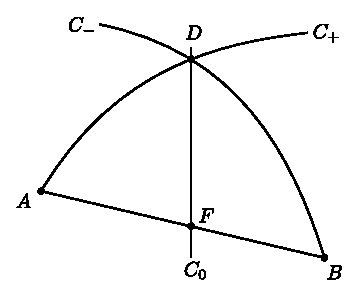
\includegraphics{figures/fig52-9.1.eps}
\caption{}\label{c9:fig9.1}
\end{figure}

Let $A$, $B$ be two nodes at which all quantities are known. We wish to calculate the various quantities at $D$ where the $C_+$ of $A$ and $C_-$ of $B$ meet. 

First we assume that $C = C(p,V)$ is a known function of $p$ and $V$. Also observe that if $(m_x, t_x)$ denotes the position of a point $X$ then, $m_D = m_F$. 

We now discretize the differential relations (\ref{eq9.32}) and (\ref{eq9.31}) (iii) and also approximate the slopes of the characteristics $C_+$ and $C_-$ to get the following equations
\begin{equation*}
\left. 
\begin{aligned}
{\rm (i)} & \qquad (u_D - u_A) + \frac{1}{2} \left(\frac{V_A}{C_A} +
\frac{V_D}{C_D}\right) (p_D - p_A) = 0\\ 
{\rm (ii)} & \qquad \frac{m_D - m_A}{t_D - t_A} = \frac{1}{2}
\left(\frac{C_A}{V_A} + \frac{C_D}{V_D}\right) 
\end{aligned}
\right\} \tag{9.33}\label{eq9.33}
\end{equation*}
for the characteristic $C_+$;
\begin{equation*}
\left. 
\begin{aligned}
{\rm (i)} & \qquad (u_D - u_B) + \frac{1}{2} \left(\frac{V_B}{C_B} +
\frac{V_D}{C_D}\right) (p_D - p_B) = 0\\ 
{\rm (ii)} & \qquad \frac{m_D - m_B}{t_D - t_B} = \frac{1}{2}
\left(\frac{C_B}{V_B} + \frac{C_D}{V_D}\right) 
\end{aligned}
\right\} \tag{9.34}\label{eq9.34}
\end{equation*}
for the\pageoriginale characteristic $C_-$;
\begin{equation*}
\epsilon_D - \epsilon_F + \frac{1}{2} (p_D+p_F) (V_D - V_F) = 0
\tag{9.35}\label{eq9.35}
\end{equation*}
for the characteristic $C_\circ$; and, 
\begin{equation*}
\epsilon_D = f(V_D, p_D)\tag{9.36}\label{eq9.36}
\end{equation*}
from the equation of state.

The equations (\ref{eq9.33}) to (\ref{eq9.36}) give six equations to
determine the six unknowns viz., $m_D, t_D, u_D, p_D, V_D,
\epsilon_D$. This non-linear system can be solved
iteratively. Assuming $V^{(0)}_D$, $p^{(0)}_D$ and hence
knowing $C^{(0)}_D$ as well, equations (\ref{eq9.33}) (ii) and
(\ref{eq9.34}) (ii) give $m^{(1)}_D$ and $t^{(1)}_D$. Simultaneously,
(\ref{eq9.33}) (i) and (\ref{eq9.34}) (i) give $u^{(1)}_D$ and
$p^{(1)}_D$. We now use (\ref{eq9.35}) and (\ref{eq9.36}) to get
$\epsilon^{(1)}_D$ and $V^{(1)}_D$. Using $V^{(1)}_D$ and $p^{(1)}_D$
we proceed to the next iteration and so on. 

One can also use the `variant' form where the points at which the solution is sought are known in advance (Cf. Sec. \ref{chap8:sec8.9}).

\section{The Method of Characteristics (with shocks)}\label{chap9:sec9.8}

Here we shall use the variant form where the points are known in
advance. We assume that there is only one shock travelling with a
positive velocity of propagation through the medium. Then to solve the
problem one must not only compute the values of the various
quantitites as the grid points but also immediately before and after
the shock at each level $n \Delta t$. The shock is pictured as the
curve $\Gamma$ in fig. \ref{c9:fig9.2}.  

\begin{figure}[H]
\centering
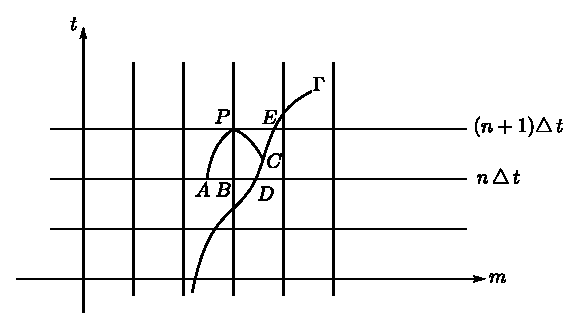
\includegraphics{figures/fig52-9.2.eps}
\caption{}\label{c9:fig9.2}
\end{figure}\pageoriginale

To compute the various quantities at an interior grid point one draws the three characteristics through this point. If none of them meets the shock before meeting the level $n\Delta t$ then we can use our previous methods for these points. If we have a point like $P$, on the other hand, where the characteristic $C_-$ meets the shock at a point $C$, then one has to use the points $A$, $B$ and $C$ in the methods of Section \ref{chap9:sec9.7}. For the values at $C$ we can interpolate these between $D$ and $E$ and thus all the grid points are tackled. 

To tackle the point $E$ where the shock meets $(n+1) \Delta t$ we proceed as follows. Our notations are now based on Fig. 9.3.

\begin{figure}[H]
\centering
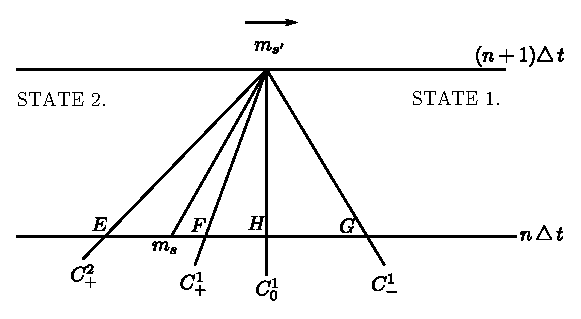
\includegraphics{figures/fig52-9.3.eps}
\centerline{Fig. 9.3}
\end{figure}\pageoriginale 

The shock meets the levels $n\Delta t$ and $(n+1)\Delta t$ at $m_s$ and $m_{s'}$ respectively. The state shead is the state 1 and the state behind is the state 2. Through $m_{s'}$ the only characteristic in state 2 is $c^2_+$. In state 1, on the other hand, all the three characteristics $C^1_+, C^1_\circ$ and $C^1_-$ exist. This is a feature of the shock. 

We then have the differential relations
\begin{equation*}
\frac{du}{ds} + \epsilon \frac{V}{C} \frac{dp}{ds} = 0
\tag{9.37}\label{eq9.37}
\end{equation*}
along $C_+$ and $C_-$ according as $\epsilon = + 1$ or $-1$, and 
\begin{equation*}
\frac{d\epsilon}{dt} + p \frac{dV}{dt} = 0
\tag{9.38}\label{eq9.38}
\end{equation*}
along $C_\circ$. We now discretize these equations.

We use the superscript 1 or 2 on the left to indicate the state in which we evaluate the various quantities. Along $C^1_-$ we have
\begin{equation*}
\left. 
\begin{aligned}
{\rm (i)} & \qquad  \frac{m_G - m_{s'}}{\Delta t} = - \frac{1}{2}
\left[{}^1 \left(\frac{C}{V}\right)_{s'} + \left(\frac{C}{V}\right)_G \right]\\ 
{\rm (ii)} & \qquad ({}^1u_{s'} - u_G ) - \left[ {}^1
  \left(\frac{v}{C}\right)_{s'} + \left(\frac{V}{C}\right)_G \right]
({}^1 p_{s'} - p_G) = 0. 
\end{aligned}
\right\}
\tag{9.39}\label{eq9.39}
\end{equation*}
Along\pageoriginale $C^1_+$ we have 
\begin{equation*}
\left.
\begin{aligned}
{\rm (i)} & \qquad \frac{m_{s'} - m_F}{\Delta t} = \frac{1}{2}
\left[{}^1 \left(\frac{C}{V}\right)_{s'} + \left(\frac{C}{V}\right)_F
  \right]\\   
{\rm (ii)} & \qquad ({}^1 u_{s'} - u_F) + \frac{1}{2} \left[{}^1
  \left(\frac{V}{C}\right)_{s'} + \left(\frac{V}{C}\right)_F \right]
({}^1 p_{s'} - p_F) = 0. \\ 
\end{aligned}
\right\}\tag{9.40}\label{eq9.40}
\end{equation*}
Along $C^1_\circ$ we have 
\begin{equation*}
{}^1 \epsilon_{s'} - \epsilon_H + \frac{1}{2} (p_H + {}^1p_{s'} ) ({}^1 V_{s'} - V_H) = 0.  
\tag{9.41}\label{eq9.41}
\end{equation*}
Along $C^2_+$ we have 
\begin{equation*}
\left. 
\begin{aligned}
{\rm (i)} & \qquad \frac{m_{s'} - m_E}{\Delta t} = \frac{1}{2}
\left[{}^2 \left(\frac{C}{V}\right)_{s'} + \left(\frac{C}{V}\right)_E \right]\\ 
{\rm (ii)} & \qquad {}^2 u_{s'} - u_E + \frac{1}{2} \left[{}^2
  \left(\frac{V}{C}\right)_{s'} + \left(\frac{V}{C}\right)_E \right]
({}^2 p_{s'} - p_E) = 0. \\ 
\end{aligned}
\right\}\tag{9.42}\label{eq9.42}
\end{equation*}

If $M  = \dfrac{dm}{dt}$ is the speed of the shock, we have the Rankine-Hugoniot relations (Cf. Sec. \ref{chap3:sec3.4})
\begin{equation*}
\left. 
\begin{aligned}
{\rm (i)} & \qquad M[V] + [u] = 0\\
{\rm (ii)} & \qquad  M[u] - [p] = 0\\
{\rm (iii)} & \qquad M[\epsilon + \frac{1}{2} u^2] - [pu] = 0\\
\end{aligned}
\right\} \tag{9.43}\label{eq9.43}
\end{equation*}
where $[\varphi] = {}^2 \varphi_{s'} - {}^1 \varphi_{s'}$ for any function $\varphi$. Also the slope of the shock is approximated by
\begin{equation*}
\frac{m_{s'} - m_s}{\Delta t} = \frac{1}{2} [M_s + M_{s'}] \tag{9.44}\label{eq9.44}
\end{equation*}

We also have the state equations
\begin{equation*}
\left.
\begin{aligned}
{\rm (i)} & \qquad {}^1\epsilon_{s'} = f({}^1 p_{s'}, {}^1 V_{s'})\\
{\rm (ii)} & \qquad {}^2 \epsilon_{s'} = f({}^2 p_{s'}, {}^2 V_{s'}). \\
\end{aligned}
\right\}
\tag{9.45}\label{eq9.45}
\end{equation*}

The\pageoriginale relations (\ref{eq9.39}) to (\ref{eq9.45}) give 13
non-linear equations. The number of unknowns is also 13, viz., the
positions $m_E, m_F, m_G, m_{s'}$, the velocity of the shock $M_{s'}$,
and the variables $u,p,V, \epsilon$ at $s'$ in states $1$ and
$2$. This system can be solved iteratively knowing all qualities at
time $n\Delta t$. We assume $M^{(0)}_{s'}$ and all the quantities
$(\frac{C}{V})^{(0)}$. Then (\ref{eq9.44}) gives
$m^{(1)}_{s'}$. Then (\ref{eq9.39}) (i) and (\ref{eq9.40}) (i) give
$m^{(1)}_G$ and $m^{(1)}_F$. We can interpolate between the grid
points at time $n\Delta t$ for the values $u^{(1)}_G$ and
$p^{(1)}_G$. Using these in (\ref{eq9.39}) (ii) and (\ref{eq9.40})
(ii) we get ${}^1 u^{(1)}_{s'}$ and ${}^1 p^{(1)}_{s'}$. Then
(\ref{eq9.41}) and (\ref{eq9.45})  (i) give ${}^1 \epsilon^{(1)}_{s'}$
and ${}^1 V^{(1)}_{s'}$. The relation (\ref{eq9.42}) (i) gives
$m^{(1)}_E$ and then by interpolation we get $p^{(1)}_E$, $u^{(1)}_E$
which we use in (\ref{eq9.42}) (ii) and (\ref{eq9.43}) (ii) to get
${}^2p^{(1)}_{s'}$ and ${}^2 u^{(1)}_{s'}$. Then (\ref{eq9.43}) (iii)
gives ${}^2 \epsilon^{(1)}_{s'}$ and finally (\ref{eq9.43}) (i) gives
$M^{(1)}_{s'}$. Now that we have $M^{(1)}_{s'}$ and both states of
$(\frac{C}{V})^{(1)}$, we can use these in the next iteration and so
on. 

\begin{remark}\label{chap9:rem9.6}
We have dealt with the case of only one shock travelling through the medium with a positive velocity. One can perform similar analysis on other types of shocks but these become very complicated. If there is an interface of two media, then a shock is transmitted into the second medium from the first and, depending on the ratio of the densities of the media, a shock may be reflected back into the first medium. In such a situation to keep track of all the shocks becomes very complicated from the logical point of view of a computer programme. 
\end{remark}

\medskip
\noindent{\textbf{REFERENCE.}}
The reader is referred to the papers of Hoskin in the Proceedings of the Conferences on Numerical Methods in Fluid Dynamics (1969, 1971, 1973 and 1975). See Roache \cite{key33} for a detailed bibliography.
